%% LyX 2.4.4 created this file.  For more info, see https://www.lyx.org/.
%% Do not edit unless you really know what you are doing.
\documentclass[english]{article}
\usepackage[T1]{fontenc}
\usepackage[latin9]{inputenc}
\usepackage{float}
\usepackage{enumitem}
\usepackage{amsmath}
\usepackage{amsthm}
\usepackage{amssymb}
\usepackage{cancel}
\usepackage{geometry}
\geometry{verbose,tmargin=1in,bmargin=1in,lmargin=1in,rmargin=1in}

\makeatletter

%%%%%%%%%%%%%%%%%%%%%%%%%%%%%% LyX specific LaTeX commands.
%% Because html converters don't know tabularnewline
\providecommand{\tabularnewline}{\\}

%%%%%%%%%%%%%%%%%%%%%%%%%%%%%% Textclass specific LaTeX commands.
\numberwithin{equation}{section}
\numberwithin{figure}{section}
\newlength{\lyxlabelwidth}      % auxiliary length 

%%%%%%%%%%%%%%%%%%%%%%%%%%%%%% User specified LaTeX commands.
\usepackage{hyperref}
\usepackage[usenames,dvipsnames,table]{xcolor} %adds additional color options
\hypersetup{colorlinks=true, urlcolor=black,linkcolor=black}

\usepackage{fancyhdr}
\usepackage{lastpage}
\pagestyle{fancy}
\usepackage{enumitem}
\usepackage{ifthen}
%sets math fonts to be more readable
\everymath=\expandafter{\the\everymath\displaystyle}
%\DeclareMathSizes{10}{10}{10}{10}
\usepackage{multicol}

\usepackage{tikz}
\usetikzlibrary{plotmarks}
\usepackage{pgfplots}
\pgfplotsset{compat=newest}

\usepackage{calc}
\usepackage[nomessages]{fp}

%\usepackage{advdate}    % Advancing/saving dates
\usepackage{datetime}   % Dates formatting
%\usepackage{datenumber} % Counters for dates
\newdateformat{MD}{\monthname[\THEMONTH] \ordinal{DAY}}

\def\formatdateny{\csname noyear\languagename\expandafter\endcsname\formatdate}
\def\noyearenglish#1, \the\@year{#1}
\let\noyearamerican\noyearenglish
\let\noyearbritish\noyearenglish

\usepackage{fancybox} %%ovalbox and fancy box settings

\usepackage[outline]{contour}  %allows text halos
\usepackage{colortbl}


\usepackage[super]{nth} %easy 1st, 2nd, etc

\usepackage{forest} %%for tree diagram

%%data for histogram%%
\begin{filecontents}{hist1_data.csv} 
dist 
3
1
0
4
1
3
2
2
0
2
0
2
2
1
4
3
1
1
3
4
2
1
3
0
1
0
2
5
1
2
3
0
0
1
2
3
1
2
0
2
\end{filecontents}

%%data for histogra: cal per cereal%%
\begin{filecontents}{hist_data_cereal.csv} 
dist 
3.7
3.6
3.6
4.0
4.0
3.6
3.8
3.7
4.1
3.9
3.9
3.3
3.5
3.6
3.9
4.0
\end{filecontents}
% Added by lyx2lyx
\setlength{\parskip}{\smallskipamount}
\setlength{\parindent}{0pt}

\makeatother

\usepackage{babel}
\begin{document}
\renewcommand{\author}{Dr.\,James Ashe}

\newcommand{\classNum}{107}

\newcommand{\classSec}{10}

\newcommand{\nameType}{Name:}

\newcommand{\examType}{Final Exam}

\renewcommand{\date}{\formatdateny{3}{12}{2014}}

%%First page's header%%%%%%%%%%%%%%%%%%%%%%
\fancypagestyle{firststyle} %%header settings for first pagr
{
	\fancyhead[L]{MTH \classNum{}(\classSec{}) \author{}\\
	\textbf{\examType{}} \date{}}
	\fancyhead[R]{\textbf{\nameType} \hspace{6cm}}
	\setlength{\headsep}{14pt}
}
%%%%%%%%%%%%%%%%%%%%%%%%%%%%%%%%%%%%%%%%%%

%%Next page's header%%%%%%%%%%%%%%%%%%%%%%%
%\setlist{nolistsep}
\lhead{MTH \classNum{}(\classSec{})} 
%\chead{\textbf{\nameType}} 
\cfoot{\thepage{}~of~\pageref{LastPage}} 
\setlength{\headsep}{5pt} 
%%%%%%%%%%%%%%%%%%%%%%%%%%%%%%%%%%%%%%%%%%%

%%Various settings; see the preamble for other settings%%%%%
%%\setenumerate[0]{leftmargin=12pt,itemindent=0pt,labelwidth=0pt}
%\setlist[2]{noitemsep}
%\setlist{nosep}
\setlist{itemsep=1pt,topsep=-5pt} %,parsep=0pt}
\setlength\multicolsep{3pt}
\renewcommand{\labelenumi}{\textbf{\arabic{enumi}.}}
\renewcommand{\labelenumii}{\textbf{\alph{enumii}.}}
\thispagestyle{firststyle}
%%%%%%%%%%%%%%%%%%%%%%%%%%%%%%%%%%%%%%%%%%
\newcommand{\xmax}{10}
\newcommand{\xmin}{-10}
\newcommand{\xstep}{0} %must be xmin+n
\newcommand{\ymax}{10}
\newcommand{\ymin}{-10}
\newcommand{\ystep}{0} %must be ymin+n

\newcommand{\xspace}{\hspace*{40pt}}
\newcommand{\yspace}{\vspace*{20pt}} %1.4cm
\newcommand{\rowColor}{gray!35}
\large\newcommand{\T}{}
\newcommand{\F}{}

\newcommand{\gauss}[2]{1/(#2*sqrt(2*pi))*exp(-((x-#1)^2)/(2*#2^2))}

\newcommand{\normalcdf}[4]{ %mean,std,z-left,z-right
\begin{tikzpicture}[scale=1.25]

\pgfmathsetmacro{\mn}{#1}
\pgfmathsetmacro{\sd}{#2}
\pgfmathsetmacro{\za}{#1+#2*1}
\pgfmathsetmacro{\zb}{#1+#2*2}
\pgfmathsetmacro{\zc}{#1+#2*3}

\pgfmathsetmacro{\zna}{#1-#2*1}
\pgfmathsetmacro{\znb}{#1-#2*2}
\pgfmathsetmacro{\znc}{#1-#2*3}

\pgfmathsetmacro{\zleft}{#3}
\pgfmathsetmacro{\zright}{#4}
\pgfmathsetmacro{\zsL}{(#3-#1)/#2} %z-score
\pgfmathsetmacro{\zsR}{(#4-#1)/#2} %z-score
\pgfmathsetmacro{\xCenter}{\zsL/2.5+\zsR/2.5} %center using z-score
\pgfmathsetmacro{\yCenter}{((1/(1*sqrt(2*pi))*exp(-((\xCenter-0)^2)/(2*1^2)))/2}
\pgfkeys{/pgf/fpu} %for large numbers
\pgfmathparse{100*(1/(1 + exp(-0.07056*((\zsR-0)/1)^3 - 1.5976*(\zsR-0)/1))-1/(1 + exp(-0.07056*((\zsL-0)/1)^3 - 1.5976*(\zsL-0)/1)))} %area from z-left to z-right
\edef\area{\pgfmathresult} 
\pgfkeys{/pgf/fpu=false}

\scriptsize
\begin{axis}[ 
	no markers, 
	domain=0:10, 
	%samples=100, 
	axis lines*=left, 
	%xlabel=Standard deviations, 
	%ylabel=Frequency, 
	height=2.5cm, %change/remove this scaling to get 1:1 pic
	width=5.5cm, 
	hide y axis,
	%ticks=none,
	xtick={-3,-2,-1,0,1,2,3},
	xticklabels={\pgfmathprintnumber[precision=0]{\znc},\pgfmathprintnumber[precision=2]{\znb},\pgfmathprintnumber[precision=2]{\zna},#1,\pgfmathprintnumber[precision=0]{\za},\pgfmathprintnumber[precision=2]{\zb},\pgfmathprintnumber[precision=2]{\zc}},
	%xticklabels={-25, -15, -5, 5, 15, 25, 35},
	%ytick=empty, 
	enlargelimits=false, 
	clip=false, 
	axis on top, 
	%grid = major
	]

	\addplot [fill=blue!35, draw=red,  domain=\zsL:\zsR] {\gauss{0}{1}} \closedcycle;
		\node (arrowEnd) at (axis cs: \xCenter, \yCenter) {};
	\addplot [draw, thick, smooth, domain=-3:3] {\gauss{0}{1}} \closedcycle;
		\node[anchor=south east] (arrowStart) at (current bounding box.east) {\pgfmathprintnumber[fixed,precision=1]{\area}\%};
	\draw[->,thick,black] (arrowStart) to (arrowEnd);
	
	%\addplot [fill=orange!20, draw=none, domain=2:3] {\gauss{0}{1}} \closedcycle; 
	%\addplot [fill=blue!20, draw=none, domain=-2:-1] {\gauss{0}{1}} \closedcycle; 
	%\addplot [fill=blue!20, draw=none, domain=1:2] {\gauss{0}{1}} \closedcycle; 
	%\only<1->{\node[above] at (axis cs: -0.5, 0.025) {$34.1\%$};} 
	%\only<1->{\node[above] at (axis cs: 0.5, 0.025) {$34.1\%$};} 
	%\only<1->{\node[above] at (axis cs: -1.5, 0.025) {$13.6\%$};}
	%\only<1->{\node[above] at (axis cs: 1.5, 0.025) {$13.6\%$};}
	%\only<1->{\node[above] at (axis cs: 2.5, 0.05) {$2.1\%$};}
	%\only<1->{\node[above] at (axis cs: -2.5, 0.05) {$2.1\%$};}
	%\only<1->{ \addplot[<->,black,very thick] coordinates {(-1,0.4) (1,0.4)};} 
	%\only<1->{\node[above] at (axis cs: 0, 0.4) {$68.2\%$};} 
	%\only<1->{\addplot[<->,black,very thick] coordinates {(-2,0.3) (2,0.3)};}
	%\only<1->{\node[above] at (axis cs: 0, 0.3) {$95.4\%$};}
	%\only<1->{\addplot[<->,black, very thick] coordinates {(-3,0.2) (3,0.2)};} 
	%\only<1->{\node[above] at (axis cs: 0, 0.2) {$99.7\%$};}
	\end{axis} 
\end{tikzpicture}
}

\newcommand{\normalpdf}[5]{ %mean,std,z-left,z-right
\begin{tikzpicture}[scale=1.25]

\pgfmathsetmacro{\mn}{#1}
\pgfmathsetmacro{\sd}{#2}
\pgfmathsetmacro{\za}{#1+#2*1}
\pgfmathsetmacro{\zb}{#1+#2*2}
\pgfmathsetmacro{\zc}{#1+#2*3}

\pgfmathsetmacro{\zna}{#1-#2*1}
\pgfmathsetmacro{\znb}{#1-#2*2}
\pgfmathsetmacro{\znc}{#1-#2*3}

\pgfmathsetmacro{\zleft}{#3}
\pgfmathsetmacro{\zright}{#4}
\pgfmathsetmacro{\zsL}{(#3-#1)/#2} %z-score
\pgfmathsetmacro{\zsR}{(#4-#1)/#2} %z-score
\pgfmathsetmacro{\zsV}{(#5-#1)/#2} %z-score
\pgfmathsetmacro{\xCenter}{\zsL/2.5+\zsR/2.5} %center using z-score
\pgfmathsetmacro{\yCenter}{((1/(1*sqrt(2*pi))*exp(-((\xCenter-0)^2)/(2*1^2)))/2}
\pgfkeys{/pgf/fpu} %for large numbers
\pgfmathparse{100*(1/(1 + exp(-0.07056*((\zsR-0)/1)^3 - 1.5976*(\zsR-0)/1))-1/(1 + exp(-0.07056*((\zsL-0)/1)^3 - 1.5976*(\zsL-0)/1)))} %area from z-left to z-right
\edef\area{\pgfmathresult} 
\pgfkeys{/pgf/fpu=false}

\scriptsize
\begin{axis}[ 
	no markers, 
	domain=0:10, 
	%samples=100, 
	axis lines*=left, 
	%xlabel=Standard deviations, 
	%ylabel=Frequency, 
	height=2.5cm, %change/remove this scaling to get 1:1 pic
	width=5.5cm, 
	hide y axis,
	%ticks=none,
	xtick={\zsV},
	xticklabels={\pgfmathprintnumber[precision=2]{#5}},
	%xticklabels={-25, -15, -5, 5, 15, 25, 35},
	%ytick=empty, 
	enlargelimits=false, 
	clip=false, 
	axis on top, 
	%grid = major
	]

	\addplot [fill=blue!35, draw=red,  domain=\zsL:\zsR] {\gauss{0}{1}} \closedcycle;
		\node (arrowEnd) at (axis cs: \xCenter, \yCenter) {};
	\addplot [draw, thick, smooth, domain=-3:3] {\gauss{0}{1}} \closedcycle;
		\node[anchor=south east] (arrowStart) at (current bounding box.east) {\pgfmathprintnumber[fixed,precision=1]{\area}\%};
	\draw[->,thick,black] (arrowStart) to (arrowEnd);
	
	%\addplot [fill=orange!20, draw=none, domain=2:3] {\gauss{0}{1}} \closedcycle; 
	%\addplot [fill=blue!20, draw=none, domain=-2:-1] {\gauss{0}{1}} \closedcycle; 
	%\addplot [fill=blue!20, draw=none, domain=1:2] {\gauss{0}{1}} \closedcycle; 
	%\only<1->{\node[above] at (axis cs: -0.5, 0.025) {$34.1\%$};} 
	%\only<1->{\node[above] at (axis cs: 0.5, 0.025) {$34.1\%$};} 
	%\only<1->{\node[above] at (axis cs: -1.5, 0.025) {$13.6\%$};}
	%\only<1->{\node[above] at (axis cs: 1.5, 0.025) {$13.6\%$};}
	%\only<1->{\node[above] at (axis cs: 2.5, 0.05) {$2.1\%$};}
	%\only<1->{\node[above] at (axis cs: -2.5, 0.05) {$2.1\%$};}
	%\only<1->{ \addplot[<->,black,very thick] coordinates {(-1,0.4) (1,0.4)};} 
	%\only<1->{\node[above] at (axis cs: 0, 0.4) {$68.2\%$};} 
	%\only<1->{\addplot[<->,black,very thick] coordinates {(-2,0.3) (2,0.3)};}
	%\only<1->{\node[above] at (axis cs: 0, 0.3) {$95.4\%$};}
	%\only<1->{\addplot[<->,black, very thick] coordinates {(-3,0.2) (3,0.2)};} 
	%\only<1->{\node[above] at (axis cs: 0, 0.2) {$99.7\%$};}
	\end{axis} 
\end{tikzpicture}
}\newcommand{\normalpdfB}[4]{ %mean,std,z-left,z-right
\begin{tikzpicture}[scale=1.25]

\pgfmathsetmacro{\mn}{#1}
\pgfmathsetmacro{\sd}{#2}
\pgfmathsetmacro{\za}{#1+#2*1}
\pgfmathsetmacro{\zb}{#1+#2*2}
\pgfmathsetmacro{\zc}{#1+#2*3}

\pgfmathsetmacro{\zna}{#1-#2*1}
\pgfmathsetmacro{\znb}{#1-#2*2}
\pgfmathsetmacro{\znc}{#1-#2*3}

\pgfmathsetmacro{\zleft}{#3}
\pgfmathsetmacro{\zright}{#4}
\pgfmathsetmacro{\zsL}{(#3-#1)/#2} %z-score
\pgfmathsetmacro{\zsR}{(#4-#1)/#2} %z-score
\pgfmathsetmacro{\xCenter}{\zsL/2.5+\zsR/2.5} %center using z-score
\pgfmathsetmacro{\yCenter}{((1/(1*sqrt(2*pi))*exp(-((\xCenter-0)^2)/(2*1^2)))/2}
\pgfkeys{/pgf/fpu} %for large numbers
\pgfmathparse{100*(1/(1 + exp(-0.07056*((\zsR-0)/1)^3 - 1.5976*(\zsR-0)/1))-1/(1 + exp(-0.07056*((\zsL-0)/1)^3 - 1.5976*(\zsL-0)/1)))} %area from z-left to z-right
\edef\area{\pgfmathresult} 
\pgfkeys{/pgf/fpu=false}

\scriptsize
\begin{axis}[ 
	no markers, 
	domain=0:10, 
	%samples=100, 
	axis lines*=left, 
	%xlabel=Standard deviations, 
	%ylabel=Frequency, 
	height=2.5cm, %change/remove this scaling to get 1:1 pic
	width=5.5cm, 
	hide y axis,
	%ticks=none,
	xtick={\zsL,\zsR},
	xticklabels={\pgfmathprintnumber[precision=2]{\zsL},\pgfmathprintnumber[precision=2]{\zsR}},
	%xticklabels={-25, -15, -5, 5, 15, 25, 35},
	%ytick=empty, 
	enlargelimits=false, 
	clip=false, 
	axis on top, 
	%grid = major
	]

	\addplot [fill=blue!35, draw=red,  domain=\zsL:\zsR] {\gauss{0}{1}} \closedcycle;
		\node (arrowEnd) at (axis cs: \xCenter, \yCenter) {};
	\addplot [draw, thick, smooth, domain=-3:3] {\gauss{0}{1}} \closedcycle;
		\node[anchor=south east] (arrowStart) at (current bounding box.east) {\pgfmathprintnumber[fixed,precision=1]{\area}\%};
	\draw[->,thick,black] (arrowStart) to (arrowEnd);
	
	%\addplot [fill=orange!20, draw=none, domain=2:3] {\gauss{0}{1}} \closedcycle; 
	%\addplot [fill=blue!20, draw=none, domain=-2:-1] {\gauss{0}{1}} \closedcycle; 
	%\addplot [fill=blue!20, draw=none, domain=1:2] {\gauss{0}{1}} \closedcycle; 
	%\only<1->{\node[above] at (axis cs: -0.5, 0.025) {$34.1\%$};} 
	%\only<1->{\node[above] at (axis cs: 0.5, 0.025) {$34.1\%$};} 
	%\only<1->{\node[above] at (axis cs: -1.5, 0.025) {$13.6\%$};}
	%\only<1->{\node[above] at (axis cs: 1.5, 0.025) {$13.6\%$};}
	%\only<1->{\node[above] at (axis cs: 2.5, 0.05) {$2.1\%$};}
	%\only<1->{\node[above] at (axis cs: -2.5, 0.05) {$2.1\%$};}
	%\only<1->{ \addplot[<->,black,very thick] coordinates {(-1,0.4) (1,0.4)};} 
	%\only<1->{\node[above] at (axis cs: 0, 0.4) {$68.2\%$};} 
	%\only<1->{\addplot[<->,black,very thick] coordinates {(-2,0.3) (2,0.3)};}
	%\only<1->{\node[above] at (axis cs: 0, 0.3) {$95.4\%$};}
	%\only<1->{\addplot[<->,black, very thick] coordinates {(-3,0.2) (3,0.2)};} 
	%\only<1->{\node[above] at (axis cs: 0, 0.2) {$99.7\%$};}
	\end{axis} 
\end{tikzpicture}
}\emph{Unless stated otherwise, all problems are worth 4 points, and
answers should be stated as decimals rounded to three decimal places.
You must show your work to receive credit. }
\begin{enumerate}[resume]
\item Using the symbolic representations\\
\begin{tabular}{rl}
$m$: & I love math.\tabularnewline
$h$: & It is hot in hades.\tabularnewline
$g$: & I went to the game.\tabularnewline
\end{tabular}\\
express the following statements in symbolic form.

\begin{enumerate}
\item I went to the game or it is hot in hades.

\begin{enumerate}
\item []\yspace\vfill
\end{enumerate}
\item If I love math then it is not hot in hades.

\begin{enumerate}
\item []\yspace\vfill
\end{enumerate}
\end{enumerate}
\item Consider the statement, ``If Theano is a woman then Theano is mortal.''
Use (a), (b), and (c) to complete parts \ref{enu:2first} and \ref{enu:2last}.

\begin{enumerate}
\item [(a)]If Theano is not a woman then Theano is not mortal. 
\item [(b)]If Theano is mortal then Theano is a woman.
\item [(c)]If Theano is not mortal then Theano is not a woman.
\item \label{enu:2first}Identify the converse of the statement. \underline{\hphantom{part a}}
\item \label{enu:2last}Identify the contrapositive of the statement. \underline{\hphantom{part a}}\vfill
\end{enumerate}
\item For parts \ref{enu:one} and \ref{enu:last}, identify the negation
of the provided statement.\newcommand{\negate}{students~}\begin{multicols}{2}

\begin{enumerate}
\item \label{enu:one}\renewcommand{\negate}{students~}Some \negate like
football.

\begin{enumerate}
\item [(a)]All \negate like football.
\item [(b)]No \negate like football.
\item [(c)]Some \negate like football.
\item [(d)]Some \negate do not like football.\vfill
\end{enumerate}
\item \label{enu:last}\renewcommand{\negate}{pilots~}All \negate can
fly a plane.

\begin{enumerate}
\item [(a)]All \negate can fly a plane.
\item [(b)]No \negate can fly a plane.
\item [(c)]Some \negate cannot fly a plane.
\item [(d)]Some \negate can fly a plane..\vfill\columnbreak
\end{enumerate}
\end{enumerate}
\end{multicols}\vfill
\item {[}8 points each{]} Use a truth table to determine if the following
arguments are valid. 

\begin{enumerate}
\item \vspace{-25pt}%
\begin{tabular}{l}
\tabularnewline
\tabularnewline
1. $q\vee r$\tabularnewline
2. $r$\tabularnewline
\hline 
$\therefore\sim q$\tabularnewline
\end{tabular}\\
\begin{tabular}{c|c|c|c|c|c|c}
\multicolumn{1}{c}{} & \multicolumn{1}{c}{} & \multicolumn{1}{c}{\ovalbox{$1$}} & \multicolumn{1}{c}{\ovalbox{$2$}} & \multicolumn{1}{c}{} & \multicolumn{1}{c}{\ovalbox{$c$}} & \ovalbox{Argument}\tabularnewline
$q$ & $r$ & $q\vee r$ & $r$ & $1 \wedge 2$ & $\sim q$ & $\left(1\wedge2\right)\rightarrow c$\tabularnewline
\hline 
\hline 
\rowcolor{\rowColor}T & T & \T & \T & \T & \F & \F\tabularnewline
\hline 
T & F & \T & \F & \F & \F & \T\tabularnewline
\hline 
\rowcolor{\rowColor}F & T & \T & \T & \T & \T & \T\tabularnewline
\hline 
F & F & \F & \F & \F & \T & \T\tabularnewline
\hline 
\multicolumn{1}{c}{} & \multicolumn{1}{c}{} & \multicolumn{1}{c}{\xspace} & \multicolumn{1}{c}{\xspace} & \multicolumn{1}{c}{\xspace} & \multicolumn{1}{c}{\xspace} & \xspace\tabularnewline
\end{tabular}\vfill\newpage
\item \vspace{-25pt} %
\begin{tabular}{rll}
 &  & \tabularnewline
 &  & \tabularnewline
$r$: & You register early. & 1. If you register early, then you will receive a discount.\tabularnewline
$d$: & You receive a discount. & 2. You register early.\tabularnewline
\cline{3-3}
 &  & Therefore, you will receive a discount.\tabularnewline
\end{tabular}\\
\begin{tabular}{c|c|c|c|c|c|c}
\multicolumn{1}{c}{} & \multicolumn{1}{c}{} & \multicolumn{1}{c}{\ovalbox{$1$}} & \multicolumn{1}{c}{\ovalbox{$2$}} & \multicolumn{1}{c}{} & \multicolumn{1}{c}{\ovalbox{$c$}} & \ovalbox{Argument}\tabularnewline
$r$ & $d$ &  &  & $1 \wedge 2$ &  & $\left(1\wedge2\right)\rightarrow c$\tabularnewline
\hline 
\hline 
\rowcolor{\rowColor}T & T & \T & \T & \T & \T & \T\tabularnewline
\hline 
T & F & \F & \T & \F & \T & \T\tabularnewline
\hline 
\rowcolor{\rowColor}F & T & \T & \F & \F & \F & \T\tabularnewline
\hline 
F & F & \T & \F & \F & \F & \T\tabularnewline
\hline 
\multicolumn{1}{c}{} & \multicolumn{1}{c}{} & \multicolumn{1}{c}{\xspace} & \multicolumn{1}{c}{\xspace} & \multicolumn{1}{c}{\xspace} & \multicolumn{1}{c}{\xspace} & \xspace\tabularnewline
\end{tabular}\vfill
\end{enumerate}
\end{enumerate}
\vfill
\begin{enumerate}[resume]
\item Let $U=\{i,l,o,v,e,m,a,t,h\}$ be the universal set, and $A=\{l,o,v,e\}$
and $B=\{v,e,m,a,th\}$ be subsets of $U$. Find the indicated set,
and draw a Venn diagram corresponding to the indicated set.\newcommand{\vennScale}{0.5}\begin{multicols}{3}

\begin{enumerate}
\item $A\cup B$\yspace\yspace\vfill
\item $A\cap B$\yspace\yspace\vfill
\item $A'$\yspace\yspace\vfill
\end{enumerate}
\end{multicols}
\item A town has $1000$ residents. Of the residents, $600$ have voted
Democrat, $500$ have voted Republican, and $200$ have voted for
both parties. \begin{multicols}{2}

\begin{enumerate}
\item Use the Venn diagram, and write the appropriate numbers in each region.
\item []%%%%A uncolored; B uncolored%%%%%
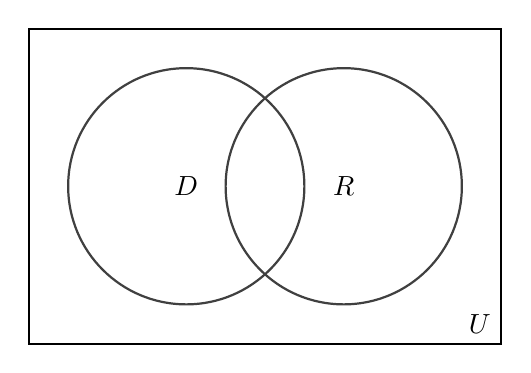
\begin{tikzpicture}[scale=1.0]
	\def\circleA{(0,0) circle (1.5)} %A
	\def\circleB{(0:2) circle (1.5)} %B

	\colorlet{circle edgeA}{black!75} 
	\colorlet{circle areaA}{red!100}
	\colorlet{circle edgeB}{black!75} 
	\colorlet{circle areaB}{green!100}

	\tikzset{
		filledA/.style={fill=circle areaA, draw=circle edgeA, thick},
		filledB/.style={fill=circle areaB, draw=circle edgeB, thick},
		outlineA/.style={draw=circle edgeA, thick},
		outlineB/.style={draw=circle edgeB, thick},
	}

	\begin{scope}[fill opacity=0.5]         
			%\fill[filledB] \circleB;    
			%\fill[filledA] \circleA;
	\end{scope}

	\draw[outlineA] \circleA node {$D$} node[below=10pt] {$$}; 
	\draw[outlineB] \circleB node {$R$} node[below=10pt] {$$}; 
	\node at (0:1) {$$}; %%intersection node%%
	\node[anchor=south] at (current bounding box.north) {$$}; 
	\draw[thick] (-2,-2) rectangle (4,2) node[anchor=south east] at (current bounding box.south east) {$U$}; 
\end{tikzpicture} \vfill\columnbreak
\item How many residents have voted Democrat but not Republican?\yspace\yspace\vfill
\item How many residents have voted Democrat or Republican?\yspace\yspace\vfill
\item How many residents have voted neither Democrat nor Republican?\yspace\yspace\vfill
\end{enumerate}
\end{multicols}\vfill
\item {[}2 pts each{]} Find the value of each of the following:\begin{multicols}{2}

\begin{enumerate}
\item $6!$\yspace\yspace\vfill
\item $\frac{10000!}{9999!}$\yspace\yspace\vfill
\item $_{6}P_{4}$\yspace\yspace\vfill
\item $_{6}C_{4}$\yspace\yspace\vfill
\end{enumerate}
\end{multicols}\newpage
\item A parking decal consists of two letters (A-Z) followed by three numbers
(0-9). If each letter and numbers can be repeated, how many different
decals can be made using this method?\yspace\yspace\vfill
\item There are $10$ pigs entered in the ``That's some pig'' contest.
How many different ways can the judges award \nth{1}, \nth{2}, and
\nth{3} place prizes?\emph{ Just write the formula}. \yspace\yspace\vfill
\item A three-person committee must be chosen from a group of three men
and four women. How many committees are possible if it must consist
of the following?\emph{ Just write the formula}. \begin{multicols}{2}

\begin{enumerate}
\item three women.\yspace\yspace\vfill
\item one man and two women.\yspace\yspace\vfill
\end{enumerate}
\end{multicols}\vfill
\item Two coins are tossed. Find each of the following:\begin{multicols}{2}

\begin{enumerate}
\item the sample space\yspace\yspace\yspace\yspace\yspace\vfill\columnbreak
\item {[}2 points{]} the event, $E_{1}$, that at least one is tails.\yspace\vfill
\item {[}2 points{]} the probability of $E_{1}$.\yspace\yspace\vfill
\end{enumerate}
\end{multicols}\vfill\newpage
\item A card is dealt from a well-shuffled, standard deck of $52$ cards.
Find the probability of being dealt each of the following:\begin{multicols}{2}

\begin{enumerate}
\item an ace of hearts\yspace\yspace\vfill\columnbreak
\item an ace or a heart\yspace\yspace\vfill
\end{enumerate}
\end{multicols}\vfill
\item A bag of candy has $10$ jelly beans. $6$ of which are red and $4$
of which are green. If you reach into the bag and randomly select
$3$ jelly beans, find the probability of the following: \emph{Just
write the formulas.}\begin{multicols}{2}

\begin{enumerate}
\item all $3$ are green.\yspace\yspace\yspace\yspace\vfill\columnbreak
\item exactly $2$ are green.\yspace\yspace\yspace\yspace\vfill
\end{enumerate}
\end{multicols}\vfill
\item Of all the residents in a town $60\%$ have voted Democrat, $50\%$
have voted Republican, and $20\%$ have voted for both parties. \begin{multicols}{2}

\begin{enumerate}
\item What is the probability that a randomly selected resident has voted
Democrat but not Republican?\yspace\vfill
\item What is the probability that a randomly selected resident has voted
Democrat or Republican?\yspace\vfill\columnbreak
\item []%%%%A uncolored; B uncolored%%%%%
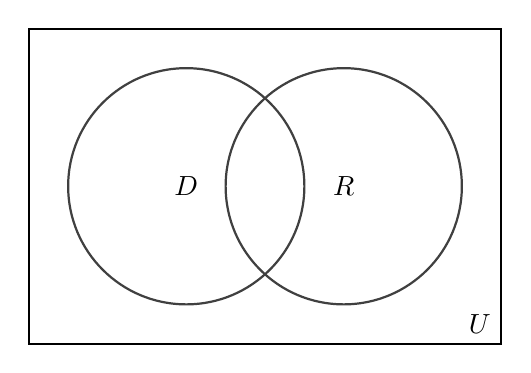
\begin{tikzpicture}[scale=1.0]
	\def\circleA{(0,0) circle (1.5)} %A
	\def\circleB{(0:2) circle (1.5)} %B

	\colorlet{circle edgeA}{black!75} 
	\colorlet{circle areaA}{red!100}
	\colorlet{circle edgeB}{black!75} 
	\colorlet{circle areaB}{green!100}

	\tikzset{
		filledA/.style={fill=circle areaA, draw=circle edgeA, thick},
		filledB/.style={fill=circle areaB, draw=circle edgeB, thick},
		outlineA/.style={draw=circle edgeA, thick},
		outlineB/.style={draw=circle edgeB, thick},
	}

	\begin{scope}[fill opacity=0.5]         
			%\fill[filledB] \circleB;    
			%\fill[filledA] \circleA;
	\end{scope}

	\draw[outlineA] \circleA node {$D$} node[below=10pt] {$$}; 
	\draw[outlineB] \circleB node {$R$} node[below=10pt] {$$}; 
	\node at (0:1) {$$}; %%intersection node%%
	\node[anchor=south] at (current bounding box.north) {$$}; 
	\draw[thick] (-2,-2) rectangle (4,2) node[anchor=south east] at (current bounding box.south east) {$U$}; 
\end{tikzpicture} \yspace\yspace\vfill
\end{enumerate}
\end{multicols}
\item A group of men and women were asked whether they preferred MacGyver
or Oprah. Use the results provided in the table to answer the following
questions.

\begin{tabular}{|c|c|c|c|}
\hline 
 & \textbf{MacGyver} & \textbf{Oprah} & \textbf{NA}\tabularnewline
\hline 
Men & 40\% & 8\% & 2\%\tabularnewline
\hline 
Women & 15\% & 30\% & 5\%\tabularnewline
\hline 
\end{tabular}\vspace{5pt}
\begin{enumerate}
\item Find the probability that a man prefers Oprah. \yspace\vfill
\item Find the probability that a person who prefers MacGyver is a women.\yspace\vfill
\end{enumerate}
\vfill\newpage
\item In Prof.\,Phails history class, $40\%$ of the students pass and
the rest fail. Of the students who fail $55\%$ are male and the rest
are female. Of the students who pass $35\%$ of the students are male
and the rest are female.\begin{multicols}{2}

\begin{enumerate}
\item draw a tree diagram describing the probability\yspace\yspace\yspace\yspace\yspace\yspace\yspace\vfill\columnbreak
\item find the probability that a student who fails is female.\yspace\vfill
\item find the probability that a student fails and is female.\yspace\yspace\yspace\vfill
\end{enumerate}
\end{multicols}\vfill
\item Use the provided raw data set to complete the following:

\hfill%
\begin{tabular}{cccccccc}
1 & 2 & 2 & 2 & 3 & 4 & 2 & 0\tabularnewline
 &  &  &  &  &  &  & \tabularnewline
 &  &  &  &  &  &  & \tabularnewline
\end{tabular}\hfill\hspace{0cm}\begin{multicols}{2}
\begin{enumerate}
\item Find the median.\yspace\yspace\vfill
\item Find the mean.\yspace\yspace\yspace\vfill\columnbreak
\item Find the mode.\vfill\yspace
\item Find the standard deviation.\vfill\yspace\yspace\yspace
\end{enumerate}
\end{multicols}\vfill
\item Create a histogram using the provided frequency distribution table.\begin{multicols}{2}

\begin{enumerate}
\item []\Large%
\begin{tabular}{|c|c|}
\hline 
\textbf{hours} & \textbf{freq.}\tabularnewline
\hline 
$0\leq x<5$ & 5\tabularnewline
\hline 
$5\leq x<10$ & 10\tabularnewline
\hline 
$10\leq x<15$ & 15\tabularnewline
\hline 
$15\leq x<20$ & 10\tabularnewline
\hline 
$20\leq x<25$ & 2\tabularnewline
\hline 
\end{tabular}\columnbreak\normalsize
\item []
\begin{figure}[H]
\centering{}
\end{figure}
\end{enumerate}
\end{multicols}\yspace\yspace\yspace\vfill\newpage
\item Find the following probabilities, \newcommand{\stretchNorm}{\vspace{110pt}}\begin{multicols}{3}

\begin{enumerate}
\item $p(z<-.81)$\stretchNorm\vfill
\item $p(z>-.81)$\stretchNorm\vfill
\item $p(-1.15<z<-.81)$\stretchNorm\vfill
\end{enumerate}
\end{multicols}
\item A population is normally distributed with mean 95 and standard deviation
10. Find the following probabilities. \begin{multicols}{2}

\begin{enumerate}
\item $p(x<80)$\stretchNorm\yspace\yspace\vfill
\item $p(x>107)$\stretchNorm\yspace\yspace\vfill
\end{enumerate}
\end{multicols}
\item Find $c$ such that each of the following is true.\begin{multicols}{3}

\begin{enumerate}
\item $p(z<c)=.6103$\stretchNorm\yspace\vfill
\item $p(z>c)=.6103$\stretchNorm\yspace\vfill
\item $p(z<c)=.43$\stretchNorm\yspace\vfill
\end{enumerate}
\end{multicols}
\item An IQ test is normally distributed with mean 100 and standard deviation
15. Find the percentage of the with a score less than $80$.\stretchNorm\vfill
\end{enumerate}

\end{document}
